\documentclass[11pt,a4paper]{report}  % Using 'report' class for structured formatting
\usepackage[utf8]{inputenc}
\usepackage{geometry}
\geometry{margin=1in}
\usepackage{graphicx}
\usepackage{setspace}
\usepackage{titlesec}
\usepackage{longtable}

\setcounter{secnumdepth}{3}
\renewcommand{\thesection}{\arabic{section}}

\begin{document}

% ------------------ Title Page ------------------

\begin{titlepage}

    \centering
   
    
\includegraphics[width=3.4cm,height=2.6cm ]{College Logo Grayscale.jpg}\\[0.5cm] % Add your college logo file

    \vspace{1cm}
    \textbf{\large A Course End Project Report on} \\[0.5cm]
    {\LARGE \textbf{Online Quiz Application}}\\[1.5cm]
 {\Large A9602 - Object Oriented Programming Laboratory}\\[1.5cm]
 \textbf{Submitted by}\\ [0.25cm]
 Batch No. 2025-OOPL-B08 

\begin{center}
	
	\begin{table}[h!]
		\centering
        \setstretch{1}
		\begin{tabular}{l l}
    
			 {Ayush Reddy AK} & {Roll No - 25881A0585}\\ [2mm]
		{G. Karthik} &  {Roll No - 25881A0586} \\ [2mm]
			 {B. Karthika} &  {Roll No - 25881A0587} \\ [2mm]
             
		\end{tabular} 
	\end{table}
\end{center}
 \textbf{Course Facilitator}\\ [0.075in]
     Ms. Jagini Padmaja\\
     Assistant Professor\\[3cm]

    { \large\textbf{Department of Computer Science and Engineering}}\\[0.5cm]
    { \large\textbf{Vardhaman College of Engineering, Hyderabad}}\\[0.5cm]
    {\large \textbf{April 2026}}

\end{titlepage}
\tableofcontents
\newpage
\noindent

\section*{Abstarct}
\noindent The Online Quiz Application is a Java-based desktop application developed using Java Swing to provide an interactive platform for conducting multiple-choice quizzes. The application allows users to register and log in using a username and password, select a subject from Java, Python, and C++, and attempt a set of multiple-choice questions.
The application provides a graphical user interface with separate screens for login, registration, subject selection, quiz participation, and result display. During a quiz, users can select one of four available options for each question, while the application automatically evaluates the selected answer and maintains the user's score. After all questions are answered, the final score is displayed to the user.
The application demonstrates the use of Java Swing components, event handling, object-oriented programming concepts, CardLayout-based screen navigation, and array-based quiz data management. It provides a simple and user-friendly approach to conducting subject-based quizzes while demonstrating the practical implementation of GUI programming concepts in Java.


\textbf{Keywords}: Java Swing, Online Quiz Application, Graphical User Interface, Multiple-Choice Quiz, Event Handling, CardLayout, Object-Oriented Programming.
\newpage
\section{Introduction}
The Online Quiz Application is a Java-based desktop application designed to provide a simple and interactive platform for conducting subject-based multiple-choice quizzes. The application is developed using Java Swing and provides a graphical user interface through which users can register, log in, select a subject, answer quiz questions, and view their final scores.
The application includes quizzes for three programming languages: Java, Python, and C++. Each subject contains a set of multiple-choice questions with four options. The application evaluates the user's selected answers and calculates the score automatically. This provides an easy way for users to test and improve their knowledge of programming concepts.
The project demonstrates several important Java programming concepts, including GUI development using Swing, event handling, object-oriented programming, arrays, conditional statements, and screen navigation using CardLayout. Different screens are provided for login, registration, subject selection, quiz participation, and result display, making the application organized and easy to use.
The main purpose of developing this application is to demonstrate the practical implementation of Java GUI programming concepts through a functional quiz system. It combines user interaction with automated answer evaluation and score calculation, providing a basic foundation that can be further expanded with features such as databases, larger question banks, user profiles, and performance tracking.

\section{Literature Review}
Online quiz applications have become a common approach for providing interactive assessment and knowledge evaluation. Traditional quizzes generally depend on paper-based questions and manual evaluation, which can require additional time and effort. Computer-based quiz systems provide an alternative by allowing questions to be presented digitally and answers to be evaluated automatically.
Java provides several features that are suitable for developing desktop-based quiz applications. In particular, the Java Swing framework provides GUI components such as buttons, labels, text fields, password fields, and panels that can be used to create interactive applications. Event handling allows the application to respond to user actions such as button clicks and option selection.
The development of a quiz application also provides an opportunity to apply fundamental programming concepts such as object-oriented programming, arrays, conditional statements, methods, and event-driven programming. In the developed application, these concepts are combined to manage user registration, login, subject selection, question navigation, answer evaluation, and score calculation.
This project focuses on implementing these concepts in a simple desktop-based quiz system. The application provides separate quizzes for Java, Python, and C++, demonstrating how a graphical interface can be combined with program logic to create an interactive learning and assessment tool.

\section{Objectives}
The main objectives of the Online Quiz Application are:
\begin{enumerate}
    \item To develop a \textbf{user-friendly graphical quiz application} using Java Swing.

    \item To implement a basic \textbf{user registration and login system} for accessing the application.

    \item To provide subject-based quizzes for \textbf{Java, Python, and C++}.

    \item To display multiple-choice questions with four answer options for each question.

    \item To automatically \textbf{evaluate the selected answers} and calculate the user's score.

    \item To provide a dedicated \textbf{result screen} that displays the user's final quiz score.

    \item To demonstrate the practical implementation of \textbf{Java Swing, event handling, arrays, methods, conditional statements, and CardLayout}.

    \item To develop a simple foundation that can be extended in the future with features such as larger question banks, database integration, user profiles, and performance tracking.
\end{enumerate}


\section{Methodology}

The Online Quiz Application was developed as a Java-based desktop application using the Java Swing framework. The methodology focuses on designing a simple graphical user interface, implementing user authentication, providing subject-based quizzes, evaluating answers, and displaying the final score. The application uses multiple screens managed through \texttt{CardLayout}, allowing the user to navigate between different stages of the application.

\subsection{System Overview}

The application consists of five main screens: Login, Registration, Menu, Quiz, and Result. The user first logs into the application using the registered credentials. New users can register by providing a username and password. After successful login, the user is taken to the main menu, where they can select one of the available subjects: Java, Python, or C++.

After selecting a subject, the corresponding set of questions and answers is loaded into the quiz screen. The user answers each question by selecting one of the four available options. The application checks the selected answer against the correct answer stored in the program and updates the score accordingly. After all questions have been answered, the final score is displayed on the result screen.

\begin{figure}[h!]
    \centering
    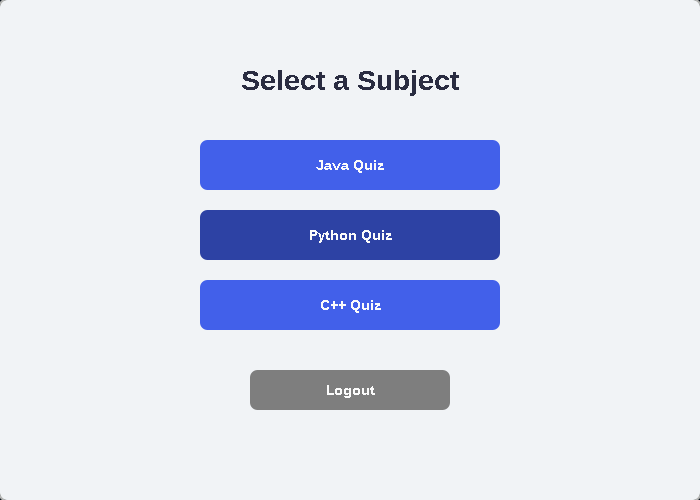
\includegraphics[width=0.9\linewidth]{screenshot-2026-10-08_22-12-10.png}
    \caption{Overall System Flow of the Online Quiz Application}
    \label{fig:system_flow}
\end{figure}

\subsection{System Flow}

The working flow of the application can be summarized as follows:

\begin{enumerate}
    \item The application starts and displays the login screen.
    \item The user enters a registered username and password.
    \item If the credentials are valid, the main menu is displayed.
    \item A new user can use the registration screen to create or update login credentials.
    \item The user selects a quiz subject from Java, Python, or C++.
    \item The application loads the questions, options, and correct answers associated with the selected subject.
    \item The user answers each question by selecting one of the four options.
    \item The selected answer is compared with the correct answer.
    \item The score is increased when the selected answer is correct.
    \item After all questions are completed, the result screen displays the final score.
    \item The user can return to the main menu and attempt another quiz or log out.
\end{enumerate}



\subsection{Main Components}

The application is divided into several functional components. Each component performs a specific task and contributes to the overall operation of the quiz system.

\subsubsection{Login and Registration Module}

The login module provides authentication using a username and password. The application initially contains a registered username and password stored in memory. When the user attempts to log in, the entered credentials are compared with the registered credentials.

If the credentials match, the application displays the main menu. Otherwise, an error message indicating invalid credentials is displayed.

The registration module allows the user to enter a new username and password. Empty username or password fields are rejected. Once valid information is entered, the registered credentials are updated in memory and the user is returned to the login screen.

\begin{figure}[h!]
    \centering
     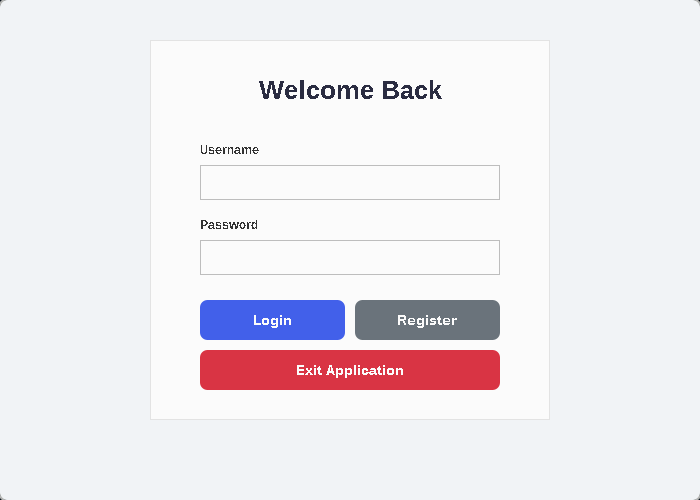
\includegraphics[width=0.9\linewidth]{screenshot-2026-10-08_22-11-35.png}
    \caption{Login Screen of the Online Quiz Application}
    \label{fig:login_screen}
\end{figure}

\begin{figure}[h!]
    \centering
     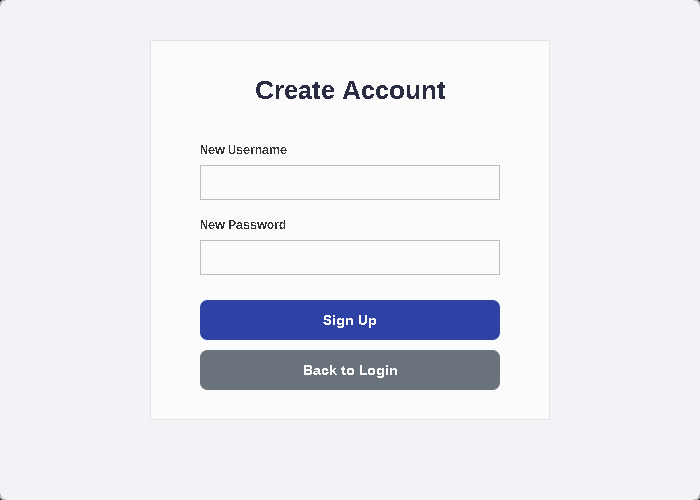
\includegraphics[width=0.9\linewidth]{screenshot-2026-10-08_22-11-46.png}
    \caption{Registration Screen of the Online Quiz Application}
    \label{fig:registration_screen}
\end{figure}

\subsubsection{Subject Selection Module}

After successful login, the user is presented with the main menu. The menu provides three quiz options: Java Quiz, Python Quiz, and C++ Quiz. Each button loads the questions and answers associated with its respective subject.

The menu also provides a logout option that returns the user to the login screen.

\begin{figure}[h!]
    \centering
     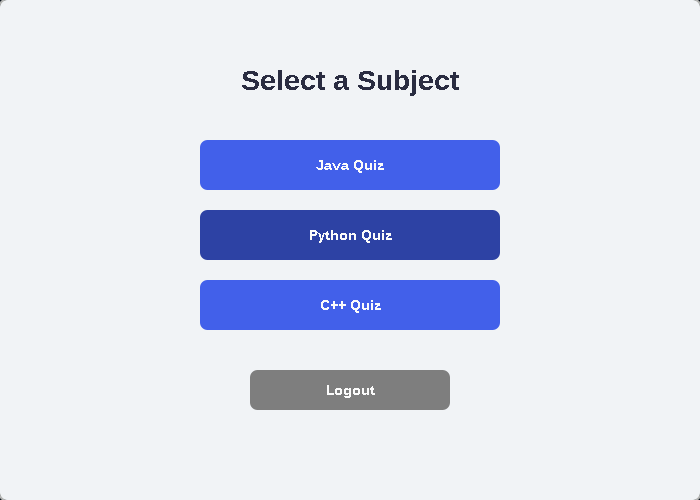
\includegraphics[width=0.9\linewidth]{screenshot-2026-10-08_22-12-10.png}
    \caption{Subject Selection Menu}
    \label{fig:subject_menu}
\end{figure}

\subsubsection{Quiz Module}

The quiz module is responsible for displaying questions and collecting the user's answers. Each quiz contains five multiple-choice questions, with four options provided for every question.

The application maintains the current question index and score using variables. The progress label indicates the current question number. When an option is selected, the application compares its index with the stored correct answer.

If the selected option is correct, the score is incremented. The application then moves to the next question. After the final question is answered, the quiz is completed and the result screen is displayed.

\begin{figure}[h!]
    \centering
     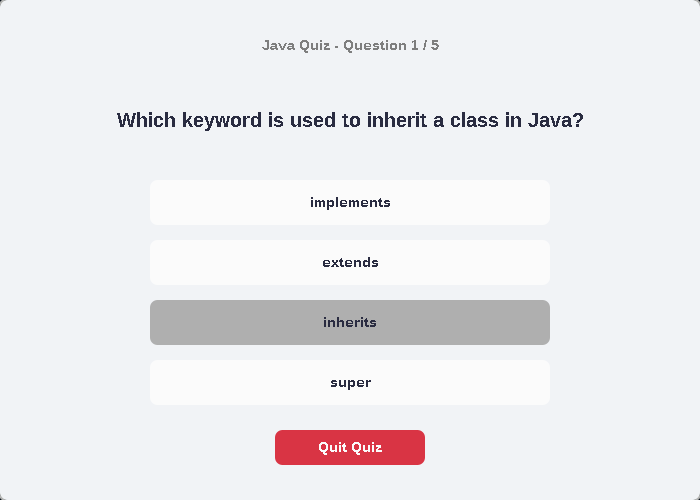
\includegraphics[width=0.9\linewidth]{screenshot-2026-10-08_22-12-17.png}
    \caption{Quiz Screen Showing a Multiple-Choice Question}
    \label{fig:quiz_screen}
\end{figure}

\subsubsection{Result Module}

After the user completes all the questions, the result module displays a completion message and the user's final score. The score is calculated based on the number of correctly selected answers.

The result screen also provides a button that allows the user to return to the main menu and select another subject.

\begin{figure}[h!]
    \centering
     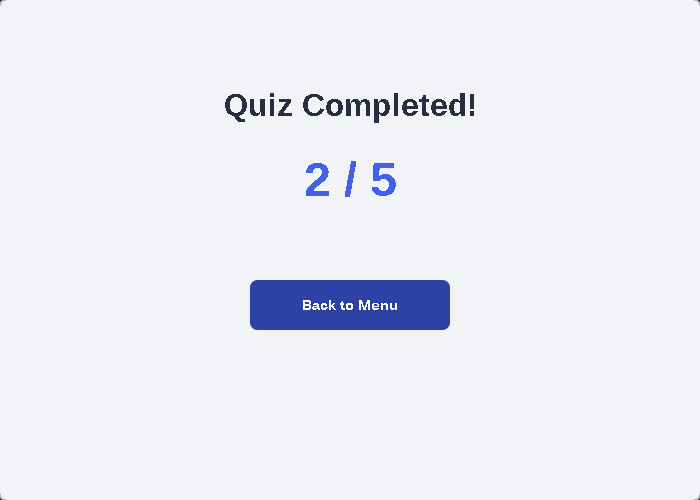
\includegraphics[width=0.9\linewidth]{screenshot-2026-10-08_22-12-27.png}
    \caption{Result Screen Showing the Final Quiz Score}
    \label{fig:result_screen}
\end{figure}

\subsection{Quiz Data}

The application contains three subject-based question sets: Java, Python, and C++. Each subject contains five questions, four options for each question, and an array containing the correct answer for every question.

When a subject is selected, the corresponding questions, options, and answer array are passed to the quiz module. The question index starts from zero and is incremented after every submitted answer.

The score is initially set to zero at the beginning of each quiz. Whenever the selected answer matches the stored correct answer, the score is increased by one.



\subsection{User Interface Design}

The graphical user interface of the application is developed using Java Swing components. The application uses labels, buttons, text fields, password fields, panels, and dialog boxes to create the different screens.

A consistent visual design is maintained throughout the application using predefined colors for the background, primary elements, text, cards, and button hover effects. The application window has a fixed size and is made non-resizable to maintain the intended layout.

A custom \texttt{ModernButton} class is also implemented by extending \texttt{JButton}. It uses \texttt{Graphics2D} to create rounded buttons and provides hover effects using mouse event handling.



\subsection{Software Implementation}

The application is implemented using Java and the Java Swing framework. The main class extends \texttt{JFrame}, which provides the main application window. Different screens are implemented as panels and are managed using \texttt{CardLayout}.

The \texttt{loadQuiz()} method loads the selected subject's questions, options, and answers while resetting the question index and score. The \texttt{updateQuizUI()} method updates the question and answer buttons displayed on the screen.

The \texttt{handleAnswer()} method processes the user's selected answer. It checks whether the selected option matches the correct answer and increases the score when appropriate. The method then advances to the next question or displays the results when the quiz is complete.

The application is launched using \texttt{SwingUtilities.invokeLater(code::new)}, ensuring that the graphical interface is created on the appropriate Swing event-dispatching thread.


\section{Results and Discussion}
 The developed Online Quiz Application successfully implements the main functions required for conducting subject-based multiple-choice quizzes. The application provides separate screens for user login, registration, subject selection, quiz participation, and result display. The use of Java Swing components provides an interactive graphical interface through which users can easily navigate between these different stages.
The login and registration modules provide basic user authentication. Users can register by entering a username and password and subsequently use those credentials to access the application. The subject selection menu allows users to choose between Java, Python, and C++ quizzes. This makes the application suitable for testing knowledge across multiple programming languages.
The quiz module successfully displays questions along with four answer options. The application maintains the current question number and score during the quiz. When a user selects an answer, it is compared with the corresponding correct answer stored in the application. Correct answers increase the score, while incorrect answers do not increase it. After all five questions are completed, the application displays the final score on the result screen.
The graphical interface uses consistent colours, buttons, labels, panels, and hover effects to provide a simple and organized user experience. The use of \texttt{CardLayout} allows the different screens to be managed within a single application window without opening multiple windows.
Overall, the application demonstrates the successful integration of Java Swing, event handling, arrays, conditional logic, methods, and object-oriented programming concepts into a functional desktop application. The current implementation provides a basic but effective quiz system. However, the application stores user credentials and quiz data in memory, meaning that the information is not permanently stored after the application is closed. This provides an opportunity for future improvements such as database integration, larger question banks, multiple user accounts, and detailed performance tracking.

\section{Mapping POs and SDGs}

\subsection{Program Outcomes}

The Online Quiz Application demonstrates the application of programming, problem-solving, and software development concepts. The following table maps the project with relevant Program Outcomes (POs).

\begin{longtable}{|p{2cm}|p{4cm}|p{8cm}|}
\hline
\textbf{PO} & \textbf{Program Outcome} & \textbf{Contribution of the Project} \\
\hline

PO1 & Engineering Knowledge & The project applies fundamental programming and software development concepts using Java and Java Swing. \\
\hline

PO2 & Problem Analysis & The project involves analyzing the requirements of a quiz system and implementing suitable logic for authentication, question handling, answer evaluation, and score calculation. \\
\hline

PO3 & Design/Development of Solutions & A graphical quiz application was designed and developed with separate modules for login, registration, subject selection, quiz participation, and result display. \\
\hline

PO5 & Modern Tool Usage & Java Swing, event handling, CardLayout, and graphical interface components are used to develop the application. \\
\hline

PO10 & Communication & The application provides clear graphical elements, labels, buttons, and messages to communicate information and instructions to the user. \\
\hline

\end{longtable}

\subsection{Sustainable Development Goals}

The project contributes to the following Sustainable Development Goals (SDGs):

\begin{longtable}{|p{2cm}|p{5cm}|p{7cm}|}
\hline
\textbf{SDG} & \textbf{Goal} & \textbf{Contribution of the Project} \\
\hline

SDG 4 & Quality Education & The application provides an interactive platform for testing programming knowledge through subject-based quizzes. \\
\hline

SDG 9 & Industry, Innovation and Infrastructure & The project demonstrates the development of a software-based digital solution using Java and graphical user interface technologies. \\
\hline

SDG 10 & Reduced Inequalities & A simple digital quiz platform can provide users with an accessible method of practicing and evaluating their programming knowledge. \\
\hline

\end{longtable}
\section{Conclusion}

The Online Quiz Application was successfully developed as a Java-based desktop application using the Java Swing framework. The application provides a simple and interactive platform for conducting multiple-choice quizzes in Java, Python, and C++. It implements important features such as user registration, login authentication, subject selection, question navigation, automatic answer evaluation, score calculation, and result display.

The project demonstrates the practical application of important Java programming concepts, including object-oriented programming, graphical user interface development, event handling, arrays, methods, conditional statements, and CardLayout-based screen navigation. The modular structure of the application makes the different stages of the quiz process easy to understand and use.

Although the current application provides the required basic functionality, it can be further improved by introducing database integration for permanent storage of users and quiz data, larger and dynamically managed question banks, multiple user accounts, user performance tracking, timers, and additional subjects. These enhancements can make the application more scalable and suitable for a larger number of users.

Overall, the project successfully demonstrates how Java programming and GUI development concepts can be combined to create a functional and user-friendly online quiz application.
%\section{References}
%\addcontentsline{toc}{section}{References}  

\begin{thebibliography}{99}
\addcontentsline{toc}{section}{Bibliography}

\bibitem{oraclejava}
Oracle Corporation,
"Java Documentation,"
Oracle. Available at:
\textit{https://docs.oracle.com/en/java/}

\bibitem{oracleswing}
Oracle Corporation,
"Creating a GUI With Swing,"
The Java Tutorials. Available at:
\textit{https://docs.oracle.com/javase/tutorial/uiswing/}

\bibitem{jframe}
Oracle Corporation,
"JFrame Class Documentation,"
Java Platform SE Documentation. Available at:
\textit{https://docs.oracle.com/javase/8/docs/api/javax/swing/JFrame.html}

\bibitem{jbutton}
Oracle Corporation,
"JButton Class Documentation,"
Java Platform SE Documentation. Available at:
\textit{https://docs.oracle.com/javase/8/docs/api/javax/swing/JButton.html}

\bibitem{cardlayout}
Oracle Corporation,
"CardLayout Class Documentation,"
Java Platform SE Documentation. Available at:
\textit{https://docs.oracle.com/javase/8/docs/api/java/awt/CardLayout.html}

\end{thebibliography}



%\begin{enumerate}
%\item Arduino Documentation. \url{https://www.arduino.cc/}
%\item HC-05 Bluetooth Module Datasheet.
%\item Research papers on wireless communication systems.
%\item MIT App Inventor Official Guide.
%\end{enumerate}
\end{thebibliography}
\end{document}